\documentclass[aspectratio=169]{beamer}
\usetheme{Madrid}
\usecolortheme{seahorse}
\usefonttheme{professionalfonts}
\usepackage[utf8]{inputenc}
\usepackage{graphicx}
\usepackage{amsmath}
\usepackage{booktabs}
\usepackage{lmodern}
\usepackage{hyperref}
\usepackage{microtype}
\usepackage{multirow}

\title[Sistema Fuzzy Mamdani]{Sistema Fuzzy Mamdani para Controle de Ventilação em Ambientes Fechados}
\author[Fabrício Silva, Leonardo Vieira Guimarães]{
    1\textsuperscript{st} Fabrício Silva \\
    \textit{Programa de Pós-Graduação em Modelagem Matemática e Computacional} \\
    \textit{CEFET-MG}
    \and
    2\textsuperscript{nd} Leonardo Vieira Guimarães \\
    \textit{Programa de Pós-Graduação em Modelagem Matemática e Computacional} \\
    \textit{CEFET-MG}
}
\institute[CEFET-MG]{Programa de Pós-Graduação em Modelagem Matemática e Computacional, CEFET-MG}
\date{\today}

\begin{document}

\begin{frame}
    \titlepage
\end{frame}

\begin{frame}{Sumário}
    \tableofcontents
\end{frame}

\section{Introdução}

\begin{frame}{Motivação}
    \begin{itemize}
        \item Ambientes fechados exigem controle eficiente de ventilação para garantir conforto térmico, qualidade do ar e economia de energia.
        \item Métodos tradicionais podem ser limitados diante das incertezas e variabilidades presentes em ambientes reais.
        \item Sistemas fuzzy, especialmente o modelo Mamdani, destacam-se por lidar com informações imprecisas e incorporar conhecimento linguístico.
    \end{itemize}
\end{frame}

\begin{frame}{Objetivo}
    \begin{itemize}
        \item Desenvolver um sistema fuzzy Mamdani para controle de ventilação em ambientes fechados.
        \item Utilizar variáveis de entrada: temperatura, umidade e número de pessoas.
        \item Demonstrar como a lógica fuzzy pode ser aplicada para tomada de decisão automática, promovendo conforto térmico e eficiência energética.
    \end{itemize}
\end{frame}

\section{Metodologia}

\begin{frame}{Universos de Discurso}
    \begin{itemize}
        \item Temperatura: 15 a 40°C \hspace{1em} (\texttt{temp\_univ = np.arange(15, 40, 0.1)})
        \item Umidade: 20 a 90\% \hspace{1em} (\texttt{umid\_univ = np.arange(20, 90, 0.1)})
        \item Pessoas: 0 a 50 \hspace{1em} (\texttt{pess\_univ = np.arange(0, 50, 0.1)})
        \item Ventilação: 0 a 100 \hspace{1em} (\texttt{vent\_univ = np.arange(0, 100, 0.1)})
    \end{itemize}
    \vspace{0.5em}
    {\small Esses intervalos garantem que o sistema fuzzy seja aplicável a diferentes ambientes e condições.}
\end{frame}

\begin{frame}{Parâmetros das Funções de Pertinência}
    \centering
    \scriptsize
    \begin{tabular}{llccc}
    \toprule
    \textbf{Variável} & \textbf{Conjunto} & \textbf{a} & \textbf{b} & \textbf{c} \\
    \midrule
    Temperatura (°C) & Baixa   & 15.00 & 21.22 & 27.45 \\
    Temperatura (°C) & Média   & 21.22 & 27.45 & 33.67 \\
    Temperatura (°C) & Alta    & 27.45 & 33.67 & 39.90 \\
    Umidade (\%)     & Baixa   & 20.00 & 37.48 & 54.95 \\
    Umidade (\%)     & Média   & 37.48 & 54.95 & 72.43 \\
    Umidade (\%)     & Alta    & 54.95 & 72.43 & 89.90 \\
    Pessoas          & Poucas  & 0.00  & 12.48 & 24.95 \\
    Pessoas          & Moderado& 12.48 & 24.95 & 37.43 \\
    Pessoas          & Muitas  & 24.95 & 37.43 & 49.90 \\
    Ventilação       & Fraca   & 0.00  & 24.98 & 49.95 \\
    Ventilação       & Moderada& 24.98 & 49.95 & 74.93 \\
    Ventilação       & Forte   & 49.95 & 74.93 & 99.90 \\
    \bottomrule
    \end{tabular}
    \vspace{0.5em}

\end{frame}

\begin{frame}{Função de Pertinência: Temperatura}
    \centering
    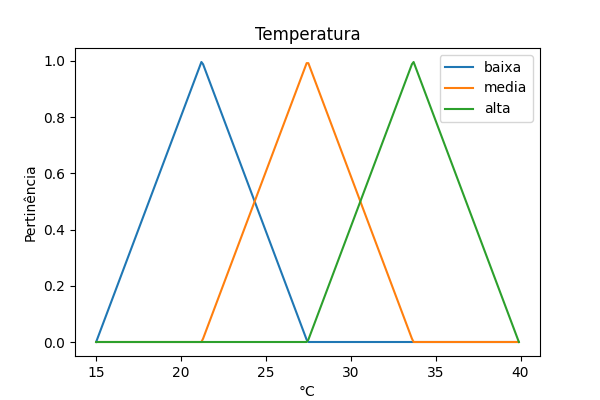
\includegraphics[width=0.7\textwidth]{../img/fp_temp_mamdani2.png}
    \vspace{0.5em}
    {\small Funções de pertinência triangulares para a variável temperatura interna.}
\end{frame}

\begin{frame}{Função de Pertinência: Umidade}
    \centering
    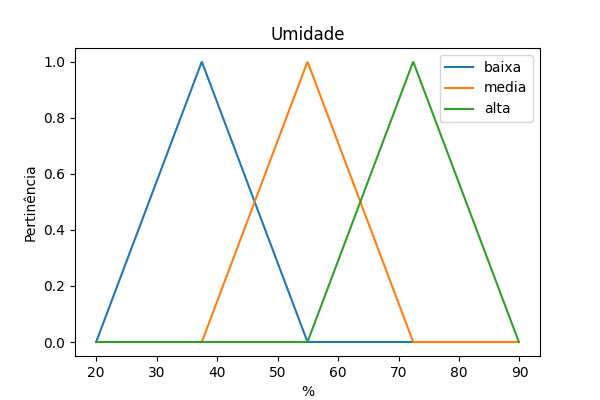
\includegraphics[width=0.7\textwidth]{../img/fp_umid_mamdani2.png}
    \vspace{0.5em}
    {\small Funções de pertinência triangulares para a variável umidade relativa.}
\end{frame}

\begin{frame}{Função de Pertinência: Pessoas}
    \centering
    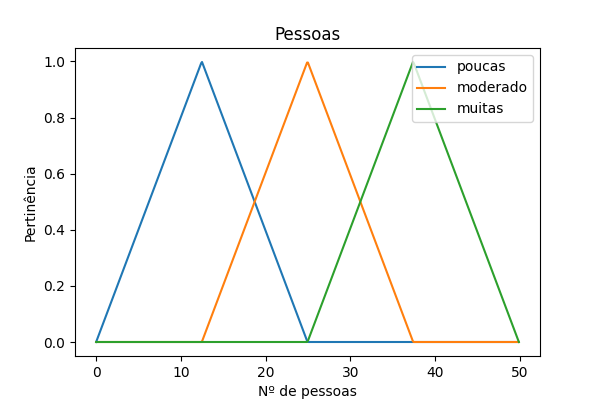
\includegraphics[width=0.7\textwidth]{../img/fp_pessoas_mamdani2.png}
    \vspace{0.5em}
    {\small Funções de pertinência triangulares para a variável número de pessoas.}
\end{frame}

\begin{frame}{Função de Pertinência: Ventilação}
    \centering
    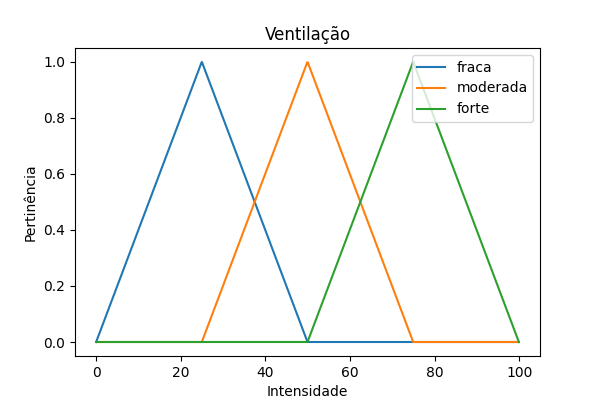
\includegraphics[width=0.7\textwidth]{../img/fp_ventilacao_mamdani2.png}
    \vspace{0.5em}
    {\small Funções de pertinência triangulares para a variável ventilação (saída).}
\end{frame}

\begin{frame}{Base de Regras Fuzzy}
    \begin{itemize}
        \item 9 regras baseadas em conforto térmico:
        \item[] Se temperatura alta OU umidade alta OU pessoas muitas então ventilação forte
        \item[] Se temperatura média E umidade média E pessoas moderado então ventilação moderada
        \item[] Se temperatura baixa E umidade baixa E pessoas poucas então ventilação fraca
        \item[] Se temperatura alta E umidade baixa então ventilação moderada
        \item[] Se temperatura média E pessoas muitas então ventilação forte
        \item[] Se umidade alta E pessoas poucas então ventilação moderada
        \item[] Se temperatura baixa OU umidade baixa então ventilação fraca
        \item[] Se pessoas moderado E umidade média então ventilação moderada
        \item[] Se temperatura média E umidade alta então ventilação forte
    \end{itemize}
\end{frame}

\begin{frame}{Cenários de Teste}
    \begin{itemize}
        \item 5 cenários simulados para avaliação do sistema.
    \end{itemize}
    \centering
    \small
    \begin{tabular}{c|c|c|c}
    \toprule
    \textbf{Cenário} & \textbf{Temperatura (°C)} & \textbf{Umidade (\%)} & \textbf{Pessoas} \\
    \midrule
    1 & 28 & 80 & 15 \\
    2 & 22 & 50 & 5  \\
    3 & 18 & 30 & 2  \\
    4 & 32 & 60 & 10 \\
    5 & 25 & 90 & 8  \\
    \bottomrule
    \end{tabular}
\end{frame}

\section{Resultados e Discussão}

\begin{frame}{Superfícies Fuzzy: Temperatura vs Umidade}
    \centering
    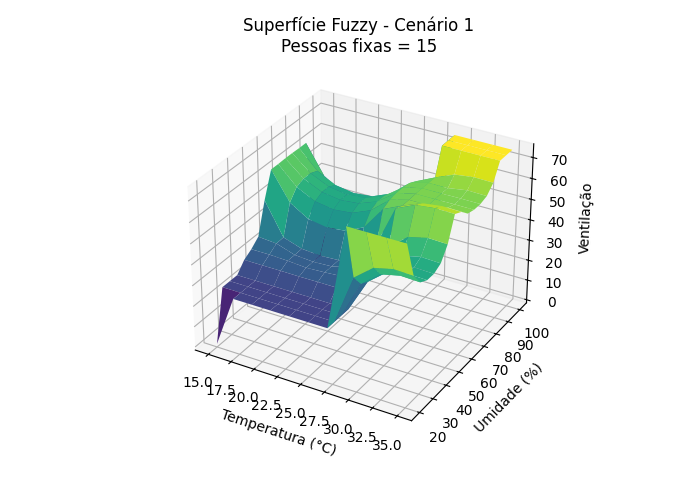
\includegraphics[width=0.7\textwidth]{../img/superficie_cenario1_fixapessoas.png}
    \vspace{0.5em}
    {\small Superfície fuzzy: ventilação em função de temperatura e umidade (pessoas fixas).}
\end{frame}

\begin{frame}{Superfícies Fuzzy: Temperatura vs Pessoas}
    \centering
    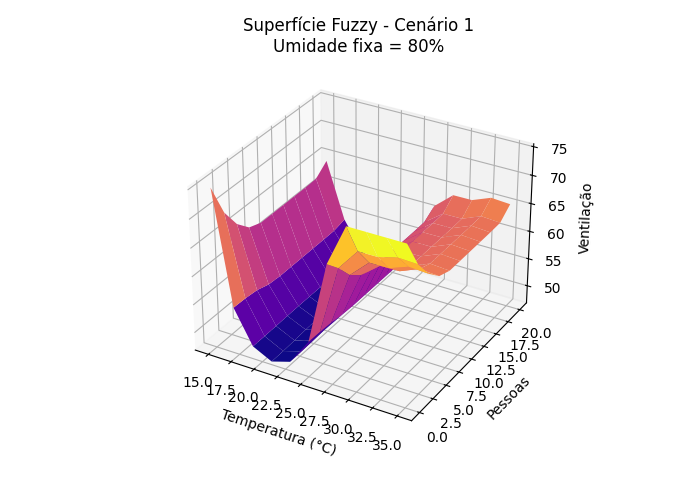
\includegraphics[width=0.7\textwidth]{../img/superficie_cenario1_fixaumidade.png}
    \vspace{0.5em}
    {\small Superfície fuzzy: ventilação em função de temperatura e pessoas (umidade fixa).}
\end{frame}

\begin{frame}{Superfícies Fuzzy: Umidade vs Pessoas}
    \centering
    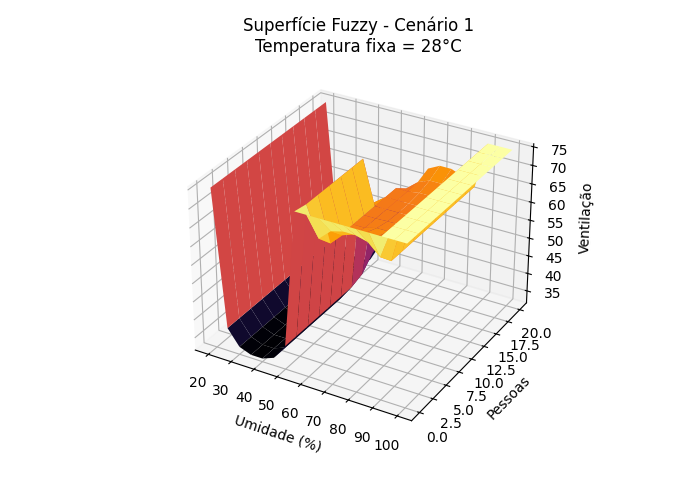
\includegraphics[width=0.7\textwidth]{../img/superficie_cenario1_fixatemperatura.png}
    \vspace{0.5em}
    {\small Superfície fuzzy: ventilação em função de umidade e pessoas (temperatura fixa).}
\end{frame}

\begin{frame}{Saída Fuzzy e Defuzzificação: Cenário 1}
    \centering
    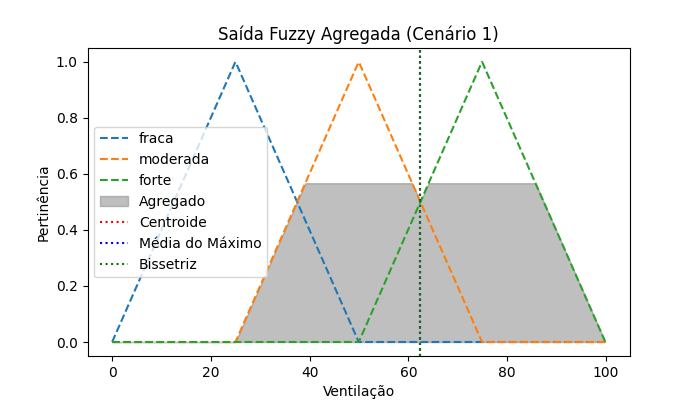
\includegraphics[width=0.7\textwidth]{../img/defuzz_cenario1.png}
    \vspace{0.5em}
    {\small Saída fuzzy agregada e valor defuzzificado para o Cenário 1.}
\end{frame}

\begin{frame}{Saída Fuzzy e Defuzzificação: Cenário 2}
    \centering
    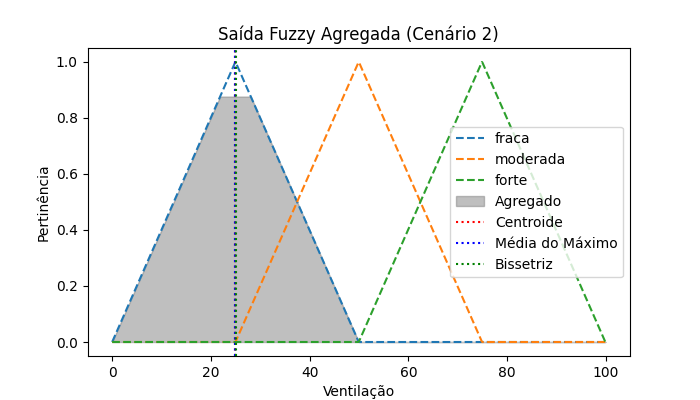
\includegraphics[width=0.7\textwidth]{../img/defuzz_cenario2.png}
    \vspace{0.5em}
    {\small Saída fuzzy agregada e valor defuzzificado para o Cenário 2.}
\end{frame}

\begin{frame}{Saída Fuzzy e Defuzzificação: Cenário 3}
    \centering
    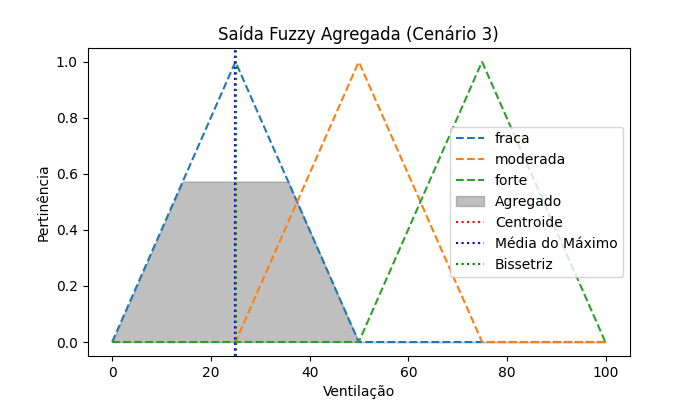
\includegraphics[width=0.7\textwidth]{../img/defuzz_cenario3.png}
    \vspace{0.5em}
    {\small Saída fuzzy agregada e valor defuzzificado para o Cenário 3.}
\end{frame}

\begin{frame}{Saída Fuzzy e Defuzzificação: Cenário 4}
    \centering
    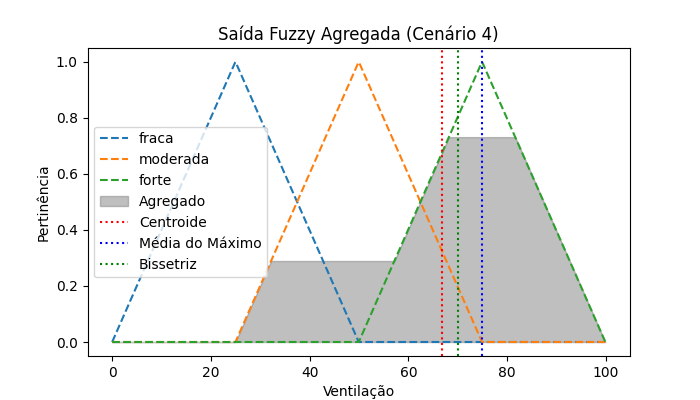
\includegraphics[width=0.7\textwidth]{../img/defuzz_cenario4.png}
    \vspace{0.5em}
    {\small Saída fuzzy agregada e valor defuzzificado para o Cenário 4.}
\end{frame}

\begin{frame}{Saída Fuzzy e Defuzzificação: Cenário 5}
    \centering
    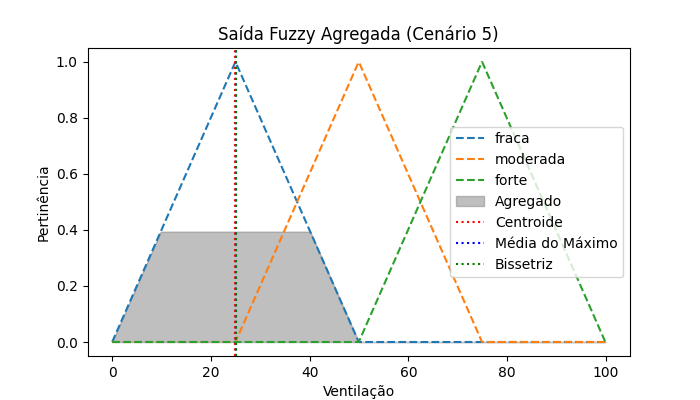
\includegraphics[width=0.7\textwidth]{../img/defuzz_cenario5.png}
    \vspace{0.5em}
    {\small Saída fuzzy agregada e valor defuzzificado para o Cenário 5.}
\end{frame}

\begin{frame}{Resumo dos Resultados Detalhado}
    \centering
    \scriptsize
    \begin{tabular}{c|c|c|c|c|l|c}
    \toprule
    \textbf{Cenário} & \textbf{Temp.} & \textbf{Umid.} & \textbf{Pessoas} & \textbf{Centroide} & \textbf{Regras Ativadas} & \textbf{Ventilação} \\
    \midrule
    1 & 28 & 80 & 15 & 62,44 & R1 (0,567), R6 (0,567), R9 (0,567) & Forte \\
    2 & 22 & 50 & 5  & 24,98 & R3 (0,283), R7 (0,876)             & Fraca \\
    3 & 18 & 30 & 2  & 24,98 & R3 (0,160), R7 (0,572)             & Fraca \\
    4 & 32 & 60 & 10 & 66,88 & R1 (0,731), R6 (0,289), R9 (0,269) & Forte \\
    5 & 25 & 90 & 8  & 24,98 & R7 (0,394)                         & Fraca \\
    \bottomrule
    \end{tabular}
\end{frame}

\begin{frame}{Discussão}
    \begin{itemize}
        \item O sistema fuzzy responde adequadamente às diferentes condições ambientais.
        \item Recomenda ventilação mais intensa para cenários com altas temperaturas, umidade elevada ou maior número de pessoas.
        \item Ventilação fraca para ambientes amenos ou pouco ocupados.
        \item Pequenas variações nos valores numéricos não afetam a tendência qualitativa das recomendações.
    \end{itemize}
\end{frame}

\section{Conclusão}

\begin{frame}{Conclusão}
    \begin{itemize}
        \item O sistema fuzzy Mamdani desenvolvido é robusto, flexível e interpretável.
        \item Fornece recomendações qualitativas de ventilação adequadas ao conforto térmico e eficiência energética.
        \item Fácil adaptação a diferentes contextos e requisitos.
        \item A escolha das funções de pertinência, operadores e técnicas de defuzzificação é fundamental para o desempenho.
    \end{itemize}
\end{frame}

\begin{frame}{Perguntas?}
    \centering
    \Huge Obrigado!
\end{frame}


\end{document}
